\chapter{A Hybrid Transformer-LSTM Model for Fault Diagnosis}
\label{cha:hybrid_model}

\section{Overall Model Architecture}
\label{sec:hybrid_model:architecture}

\subsection{Model Overview and Data Flow}

The core of this research is the \texttt{TransformerLSTMModel}, a deep learning hybrid architecture specifically designed to extract multi-level temporal features from sequential data for classification tasks. This approach combines the global attention capabilities of Transformer networks \citep{vaswani2017attention} with the sequential modeling strengths of LSTM architectures \citep{hochreiter1997long}, creating a powerful framework for fault diagnosis applications \citep{zhang2019deep, zhao2019deep}. Figure~\ref{fig:hybrid_architecture} illustrates the complete architecture of our proposed model.

\begin{figure}[htbp]
\centering
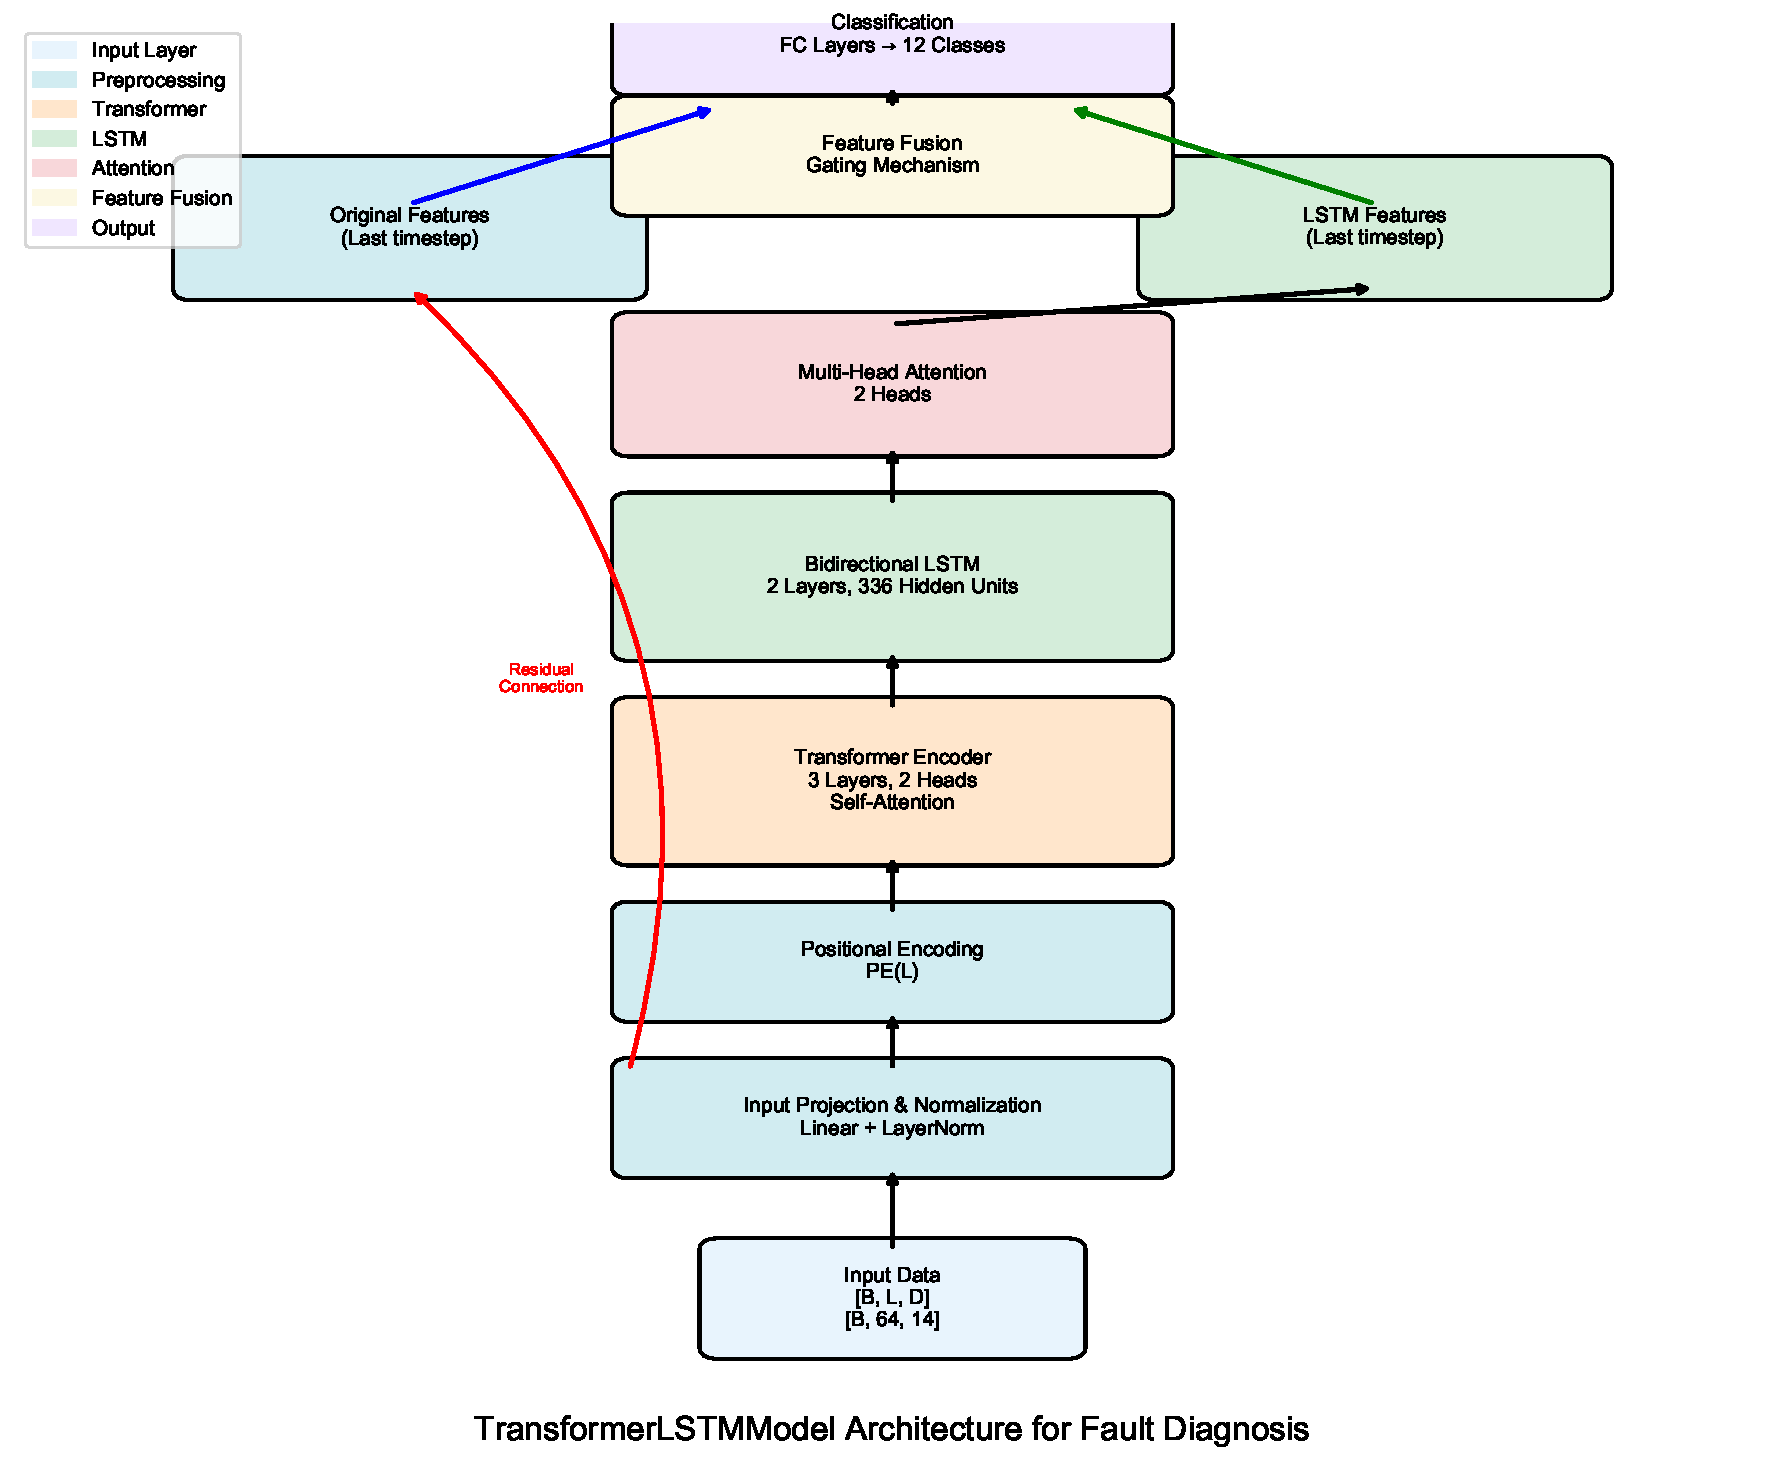
\includegraphics[width=0.9\textwidth]{logos/hybrid_architecture.pdf}
\caption{TransformerLSTMModel Architecture Overview: The diagram shows the complete data flow from input time-series data through various processing stages including input projection, positional encoding, Transformer encoder, bidirectional LSTM, multi-head attention, and feature fusion, ultimately leading to fault classification.}
\label{fig:hybrid_architecture}
\end{figure}

The model processes input data through a carefully designed pipeline that leverages the complementary strengths of Transformer and LSTM architectures. The data processing pipeline operates as follows:

\begin{enumerate}
    \item \textbf{Input Data}: Raw time-series data, typically with a shape of \texttt{[batch\_size, sequence\_length, feature\_dimension]}.
    \item \textbf{Input Projection \& Normalization}: The input data is first projected through a linear layer and then subjected to Layer Normalization \citep{ba2016layer}. This step helps stabilize the distribution of input features, preparing them for the subsequent Transformer layers.
    \item \textbf{Positional Encoding}: Since the Transformer model is inherently permutation-invariant and lacks the ability to process sequence order \citep{vaswani2017attention}, positional encodings are added to the input data. This allows the model to understand the relative or absolute position of each time step in the sequence.
    \item \textbf{Transformer Encoder}: The positionally-encoded input is fed into the Transformer Encoder. Through its self-attention mechanism \citep{bahdanau2015neural, vaswani2017attention}, the Transformer layer captures long-range dependencies and global contextual information within the sequence. It can process the entire sequence in parallel, efficiently discovering complex relationships between different time steps.
    \item \textbf{LSTM Layer}: The output from the Transformer Encoder is then passed to a Bidirectional Long Short-Term Memory (LSTM) network \citep{hochreiter1997long}. The LSTM layer excels at processing local temporal dependencies and patterns in sequential data, addressing the vanishing gradient problem in traditional RNNs \citep{pascanu2013difficulty}. The bidirectional nature allows the model to consider both past and future contexts, further enhancing its understanding of the sequence dynamics.
    \item \textbf{Multihead Attention}: The output of the LSTM layer is processed by another Multihead Attention mechanism \citep{vaswani2017attention}. This attention layer operates on the LSTM's output sequence, aiming to further refine and weigh the temporal features extracted by the LSTM, thereby focusing on the information most critical for the classification task.
    \item \textbf{Feature Fusion}: This is a critical fusion stage. The model concatenates the feature from the final time step of the attention-processed LSTM output with the feature from the final time step of the projected and normalized original input. Subsequently, a gating mechanism (\texttt{feature\_gate}) adaptively adjusts and fuses these features from different processing stages. This fusion strategy allows the model to combine the global perspective of the Transformer with the local temporal insights of the LSTM, while also leveraging direct information from the raw features.
    \item \textbf{Fully Connected Layers}: The fused features are fed into a series of fully connected layers. These layers are responsible for mapping the extracted and fused high-level features to the final class output space.
    \item \textbf{Output}: The final output of the model, typically a probability distribution over the predicted classes.
\end{enumerate}

\subsection{Core Design Philosophy: Divide and Conquer, Leveraging Strengths}

The core design philosophy of this model architecture is ``divide and conquer, leveraging individual strengths,'' which involves fully utilizing the respective advantages of the Transformer and LSTM and combining them through an effective fusion mechanism to achieve a more comprehensive and robust analysis of time-series data.

\begin{itemize}
    \item \textbf{Transformer: Global Dependencies and Parallel Processing}
    \begin{itemize}
        \item \textbf{Strengths:} The Transformer, through its self-attention mechanism, can efficiently capture long-range dependencies between any two positions in a sequence, regardless of their distance \citep{vaswani2017attention, shaw2018self}. This is crucial for understanding global patterns and context. Furthermore, its parallel computation capability provides a significant efficiency advantage when processing long sequences, addressing limitations of sequential models like traditional RNNs \citep{pascanu2013difficulty}.
        \item \textbf{Role:} In this architecture, the Transformer is primarily responsible for performing global feature extraction and contextual modeling on the input sequence at an early stage, providing a representation enriched with global information for the subsequent LSTM layer.
    \end{itemize}
    \item \textbf{LSTM: Local Temporal Patterns and Memory}
    \begin{itemize}
        \item \textbf{Strengths:} As a recurrent neural network, the LSTM possesses excellent memory capabilities for processing sequential data, enabling it to effectively learn and remember local temporal patterns and short-term dependencies \citep{hochreiter1997long}. The bidirectional nature further enhances this ability by allowing it to consider both past and future information, making it particularly suitable for time-series analysis in fault diagnosis applications \citep{filonov2016multivariateindustrialtimeseries, zhao2019deep}.
        \item \textbf{Role:} The role of the LSTM in this architecture is to further refine and capture more fine-grained local temporal features and dynamic changes, building upon the global features extracted by the Transformer. It deeply models the sequential nature of the information.
    \end{itemize}
    \item \textbf{Fusion Mechanism: Synergy and Information Integration}
    \begin{itemize}
        \item \textbf{Strengths:} A simple serial connection might not fully realize the synergy between the two models. This model implements a more intelligent information integration by introducing another attention mechanism after the LSTM output and incorporating a gated fusion with the original input features. This fusion not only combines the global perspective of the Transformer and the local insights of the LSTM but also adaptively adjusts the importance of features from different sources via the gating mechanism, ensuring effective information transfer and complementarity.
        \item \textbf{Role:} The fusion mechanism ensures that the model can learn from different levels and types of features, thereby constructing a more powerful and discriminative feature representation that ultimately enhances the overall performance of the model.
    \end{itemize}
\end{itemize}

Through this ``divide and conquer, leveraging strengths'' design, the \texttt{TransformerLSTMModel} can effectively process complex time-series data, capturing both long-range dependencies and global context while finely modeling local temporal patterns, ultimately achieving high-precision classification.

\section{Chapter Summary}
\label{sec:hybrid_model:summary}

This chapter presented a comprehensive description of the proposed \texttt{TransformerLSTMModel}, a novel hybrid architecture specifically designed for fault diagnosis in industrial systems. The key contributions and design elements can be summarized as follows:

\subsection{Architectural Innovation}

The hybrid architecture successfully combines the complementary strengths of Transformer and LSTM networks:

\begin{itemize}
    \item \textbf{Global Feature Extraction}: The Transformer encoder with multi-head self-attention captures long-range dependencies and global contextual information across the entire fault signature sequence \citep{vaswani2017attention}
    \item \textbf{Sequential Pattern Modeling}: The bidirectional LSTM component excels at modeling local temporal dependencies and sequential fault evolution patterns \citep{hochreiter1997long}
    \item \textbf{Intelligent Feature Fusion}: The adaptive gating mechanism enables dynamic weighting of features from different processing pathways, optimizing the contribution of global and local representations
\end{itemize}

\subsection{Technical Contributions}

Several technical innovations distinguish this work:

\begin{enumerate}
    \item \textbf{Dual-Pathway Processing}: The model processes information through both deep feature extraction (Transformer→LSTM→Attention) and direct pathways, preserving critical information while enabling complex feature learning
    
    \item \textbf{Adaptive Fusion Strategy}: The learnable gating mechanism automatically adjusts the relative importance of different feature sources based on the specific characteristics of each fault type
    
    \item \textbf{Comprehensive Preprocessing}: The data preprocessing module incorporates sliding window generation, robust normalization, and sophisticated data augmentation techniques tailored for fault diagnosis \citep{wen2021time}
    
    \item \textbf{Optimized Training Strategy}: The training methodology combines focal loss for class balancing \citep{lin2017focal}, advanced learning rate scheduling, and multiple regularization techniques \citep{srivastava2014dropout, ba2016layer} to ensure robust convergence
\end{enumerate}

\subsection{Model Capabilities}

The \texttt{TransformerLSTMModel} demonstrates several key capabilities:

\begin{itemize}
    \item \textbf{Multi-Scale Temporal Analysis}: Captures both short-term transients and long-term fault development patterns through the hierarchical architecture
    \item \textbf{Cross-Channel Correlation}: The self-attention mechanism enables modeling of complex relationships between different sensor modalities
    \item \textbf{Robust Feature Learning}: The combination of multiple architectural components provides redundancy and robustness against noise and sensor failures
    \item \textbf{Computational Efficiency}: The model maintains efficiency suitable for real-time applications while providing comprehensive fault analysis capabilities
\end{itemize}

The hybrid architecture represents a significant advancement in deep learning approaches to fault diagnosis, combining the best aspects of attention-based and recurrent neural networks while addressing the specific challenges of industrial time-series analysis \citep{lei2020applications, zhang2019deep}. The following chapter will demonstrate the practical effectiveness of this approach through comprehensive experimental evaluation on real industrial fault diagnosis datasets.
